
\chapter{Referencial Teórico} \label{cap:funda}

\vspace{-2cm} %Deixar no formato certo, 1 'ENTER' após e a seção e 2 'ENTERs' antes da seção

Neste capítulo são apresentados os principais conceitos teóricos relacionados ao desenvolvimento deste trabalho.


%%%%%%%%%%%%%%%%%%%%%%%%%%%%%%%%%%%%%%%%%%%%%%%%%%%%%%%%%%%%%%%%%%%%%%%%%%%%%%%%%%%%%%%%%%%%%%%%%%%%%%%%%%%%%%%%%%%%%%%%%%
\vspace{1cm}
\section{Robótica} \label{cap:rob_auto}
% Passar pra frente
A palavra ``Robô'' foi criada pelo escritor tcheco Karel Capek, sendo utilizada em sua peça 
\textit{Rossum's Universal Robots} (\sigla{RUR}{\textit{Rossum's Universal Robots}}), a qual foi 
encenada em 1921, em Praga. Na linguagem eslava, \textit{robota} significa atividade 
forçada ou escrava. Na peça de Capek, os robôs eram pessoas fabricadas artificialmente, ausentes
de emoção \cite{polonskii1996}.\par
A \textit{Robotic Industries Association} (\sigla{RIA}{\textit{Robotic Industries Association}}), 
entidade norte-americana responsável pela indústria de robótica, define um robô industrial como
 \textit{um manipulador multipropósito reprogramável, controlado automaticamente, programado em três 
 ou mais eixos, os quais podem ser fixos em um lugar ou móveis para aplicações em automação industrial} \cite{RIAdef}.
%\footnote{Fonte em \url{http://www.robotics.org/product-catalog-detail.cfm/productid/2953}. Acesso em: 15 agosto 2016}. 
%Diferentemente do que foi imaginado por Capek, hoje máquinas fazem o trabalho destes seres-humanos.
Diferentemente do que foi imaginado por Capek, são máquinas que realizam o trabalho.

%\begin{comment}
\citeonline{secchi2012} classifica os robôs em três tipos:
\begin{itemize}
 \item Industriais: São formados por estruturas mecâncias articuladas, as quais se movem pelas ordens de um sistema de 
 controle, normalmente um microcontrolador;
 \item Médicos: Também conhecidos como de cooperação ou reabilitação, são os utilizados em cirurgias de alta complexidade e 
 precisão, assim como as próteses inteligentes, que visam manter a aparência e funcionalidade do membro de pessoas com 
 deficiência.;
 \item Móveis: São plataformas mecânicas, que se locomovem através de um certo ambiente e apresentam certa autonomia.
São empregados principalmente em tarefas onde se tem risco à vida humana, como na manutenção de reatores nucleares ou 
exploração de 
minérios, mas também podem ser aplicados na agricultura e no transporte de cargas.
\end{itemize}


\vspace{1cm}
%\subsection{Robôs móveis}
\subsection{Robótica móvel}	


Mesmo que os robôs industriais apresentem alta precisão e velocidade, estes possuem uma grande desvantagem, que é a falta 
de mobilidade. %Algumas atividades necessitam que o dispositivo trafeguem através de uma planta industrial
Algumas atividades não seriam realizadas sem a utilização destes dispositivos, como a 
\textit{Mars Pathfinder}, missão exploratória da 
\sigla{NASA}{ \textit{National Aeronautics and Space Administration}} para o reconhecimento da atmosfera de Marte. O 
veículo Sojourner (Figura \ref{fig:nasa}) que foi utilizado nesta missão, explorou o território marciano por 83 dias, 
tirando fotografias e realizando 
medições do ambiente \cite{nasa}.

\begin{figure}[th]
 \centering
 \captionsetup{width=0.5\textwidth,font=footnotesize,textfont=bf}
 %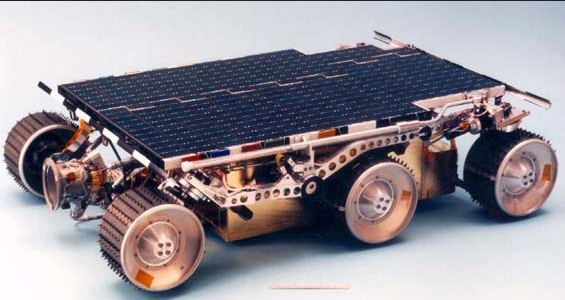
\includegraphics[scale=0.6]{figuras/nasa.png}
 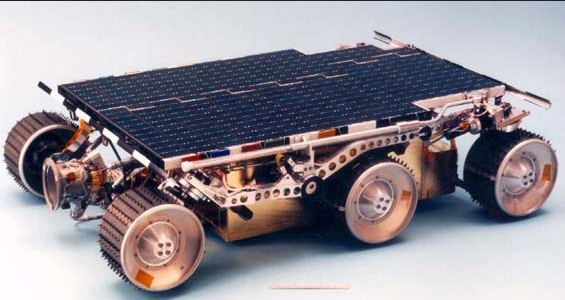
\includegraphics[scale=0.4]{figuras/nasa.png}
 \caption{Veículo exploratório Sojourner \label{fig:nasa}}
 \vspace{-0.3cm}
 %\caption*{Fonte: Disponível em \url{https://mars.jpl.nasa.gov/MPF/rover/sim2.jpg}.}
 \caption*{Fonte: Disponível em $<$https://mars.jpl.nasa.gov/MPF/rover/sim2.jpg$>$}
\end{figure}


A robótica móvel lida com o controle de veículos autônomos e semi-autônomos, tendo ênfase em problemas relacionados com o 
espaço em larga escala, que são regiões com espaços consideravelmente maiores que as observáveis pelo ponto de visão 
do robô. O espaço em larga escala é de extrema importância para um robô móvel, visto que afeta 
o seu movimento, compreensão e raciocínio nesta área, sendo estes três subproblemas essenciais para este campo de pesquisa
\cite{dudek_mobile}.

%\cite{nasa}
%É uma área de pesquisa interdisciplinar, consistindo de ...

\begin{comment}
% Retirado do livro do dudek
A mobile robot is a combination of various physical (hardware) and computational (soft-
ware) components. In terms of hardware components, a mobile robot can be considered
as a collection of subsystems for:
Locomotion: How the robot moves through its environment
Sensing: How the robot measures properties of itself and its environment
Reasoning: How the robot maps these measurements into actions
Communication: How the robot communicates with an outside operator
Later chapters consider the algorithms and representations that make these capabilities
possible, while this chapter concentrates on the underlying hardware, with special empha-
sis on locomotion for wheeled robots.
\end{comment}


%  No mean feat, this makes
%mobile robotics as interdisciplinary a field as there can be. To solve locomotion problems,
%the mobile roboticist must understand mechanism and kinematics, dynamics and control
%theory. To create robust perceptual systems, the mobile roboticist must leverage the fields
%of signal analysis and specialized bodies of knowledge such as computer vision to properly
%employ a multitude of sensor technologies. Localization and navigation demand knowl-
%edge of computer algorithms, information theory, artificial intelligence, a
  
\citeonline{Intro_auto} classifica os robôs móveis em duas categorias relacionadas à locomoção: 
\begin{itemize}
 
 \item Robôs terrestres (\textit{legged robots}): Tem como vantagem a manipulação de objetos e a locomoção em terrenos 
acidentados, mas tem alta complexidade mecânica e energética. A Figura \ref{fig:boston} mostra o 
\textit{Legged Squad Support Systems} (\sigla{LS3}{\textit{Legged Squad Support Systems}}) da Boston Dynamics, 
projetado para atuar nos mesmos terrenos acidentados utilizados por \textit{marines} e soldados norte-americanos, 
ajudando a carregar equipamentos \cite{bostondyn}. 
\begin{figure}[h]
 \centering
 \captionsetup{width=0.44\textwidth,font=footnotesize,textfont=bf}
 %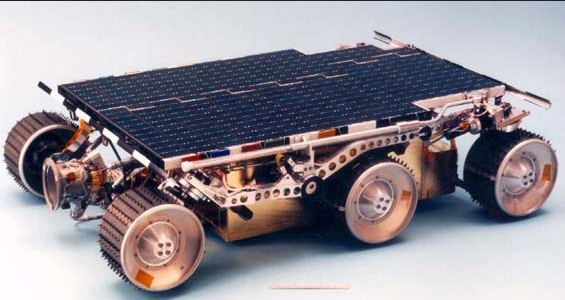
\includegraphics[scale=0.6]{figuras/nasa.png}
 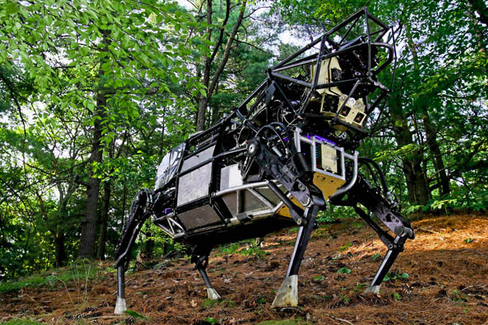
\includegraphics[scale=0.4]{figuras/bostondyn.png}
 \caption{Robô terrestre  L3S\label{fig:boston}}
 \vspace{-0.3cm}
 \caption*{Fonte: \cite{bostondyn}}
\end{figure}


\item Robôs com rodas (\textit{wheeled robots}): É tipo de locomoção mais utilizado em robôs móveis e veículos. Normalmente o 
equilíbrio não é levado em consideração, visto que na maior parte dos projetos as rodas são consideradas em contato com o solo 
o tempo todo. O robô Sojourner da Figura \ref{fig:nasa} é um exemplo de robô com rodas.

\end{itemize}

%Dentre os robôs com rodas, a categoria dos seguidores de linha tem destaque.
Os seguidores de linha, categoria pertencente aos robôs com rodas, serão abordados na próxima subseção.


\subsubsection{Robôs seguidores de linha}

Os robôs seguidores de linha são projetados para seguirem um trajeto, o qual normalmente é feito por marcações no solo. 
Estes veículos são bastante utilizados devido ao seu baixo custo e simplicidade de projeto \cite{lfchina}.





%%%%%%%%%%%%%%%%%%%%%%%%%%%%%%%%%%%%%%%%%%%%%%%%%%%%%%%%%%%%%%%%%%%%%%%%%%%%%%%%%%%%%%%%%%%%%%%%%%%%%%%%%%%%%%%%%%%%%%%%%%
\vspace{1cm}
\section{Sistema embarcado}

%Segundo Li e Qual (sei lá? 2008), um sistema embarcado é \textit{Um sistema embarcado é um sistema BLABLABLA... continua}.
Sistemas embarcados são sistemas computacionais que integram \textit{harware} e \textit{software}, com o objetivo de 
rodar uma aplicação específica \cite{embedded}.

%%%%%%%%%%%%%%%%%%%%%%%%%%%%%%%%%%%%%%%%%%%%%%%%%%%%%%%%%%%%%%%%%%%%%%%%%%%%%%%%%%%%%%%%%%%%%%%%%%%%%%%%%%%%%%%%%%%%%%%%%%%
\vspace{1cm}
\section{Regras da Robocore para robôs seguidores de linha} \label{cap:regras_comp}

Na Seção \ref{cap:espc_robocore} e Seção \ref{cap:perc_robocore} são apresentadas as regras relacionadas à 
especificação dos robôs e do percurso, respectivamente, 
para a categoria robô seguidor de linha Pro, em eventos realizados pela \citeonline{RegrasRobocore}.

\vspace{1cm}
\subsection{Especificação dos robôs} \label{cap:espc_robocore}

Para competir na categoria seguidor de linha, os robôs devem ser totalmente autônomos, não podendo ser controlados 
externamente por fio ou por rádio, com exceção para quando este for iniciado. Todos os componentes devem ser embarcados. A 
dimensão máxima permitida é de 250mm   de   comprimento,   250mm   de   largura   e   200mm   de   altura. Não é 
permitido alterar as dimensões do robô durante a partida, assim como alterar o \textit{hardware} ou \textit{software} 
durante a tomada de tempo. Também não é permitida a utilização de mecanismo de sucção, 
que vise aumentar a força normal do robô em relação ao solo.

\vspace{1cm}
\subsection{Especificações do Percurso} \label{cap:perc_robocore}

A pista é feita de uma ou mais placas de \sigla{MDF}{\textit{Medium-Density Fiberboard}} revestidas com uma manta de 
borracha preta, assim, eventualmente serão necessárias emendas para compor a área do percurso. Os robôs, no entanto, 
devem ser capazes de superar os desníveis decorrentes das emendas, que são de aproximadamente 1mm.
Uma linha branca, de 19$\pm$1mm, indica o percurso. Esta linha pode cruzar sobre ela mesma, tendo, neste caso, 
um ângulo de intersecção de 90$\pm$5º (graus), com os 250mm antes e depois do cruzamento sendo retas (conforme pode 
ser visto na Figura \ref{fig:percurso1}). O circuito é totalmente plano, porém podem ocorrer 
inclinações de até 5º.\par



\begin{figure}[h!]
 \centering
 \captionsetup{width=0.37\textwidth,font=footnotesize,textfont=bf}
 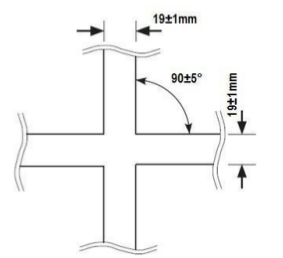
\includegraphics[scale=0.6]{figuras/Percurso1.png}
 \caption{Intersecções no percurso \label{fig:percurso1}}
 \vspace{-0.7cm}
 \caption*{Fonte: Disponível em \cite[p.4]{RegrasRobocore}.}
\end{figure}
%\captionsetup{width=0.50\textwidth, font=footnotesize, textfont=bf}






A área que se estende entre o ponto de partida e o ponto de chegada, considerando 200mm da linha e 200mm a esquerda da linha
 é denominada ``área de partida-chegada'', conforme pode ser visto na Figura \ref{fig:percurso2}.\par

\vspace{0.6cm}
\begin{figure}[h!]
 \centering
 \captionsetup{width=0.55\textwidth,font=footnotesize,textfont=bf}
 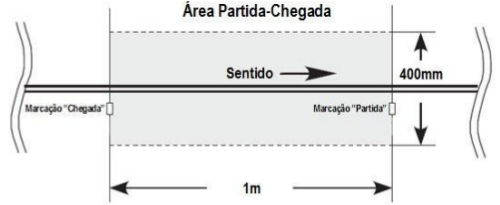
\includegraphics[scale=0.5]{figuras/Percurso2.png}
 \caption{Área de partida-chegada \label{fig:percurso2}}
  \vspace{-0.3cm}
 \caption*{Fonte: Disponível em \cite[p.4]{RegrasRobocore}.}
\end{figure}



%\captionsetup{width=0.50\textwidth, font=footnotesize, textfont=bf}
Quando houver um arco (intersecção entre a faixa branca), o raio deste é de pelo menos 100mm. Quando houver uma 
alteração na curvatura do percurso, deve haver uma marcação no lado esquerdo da linha, como pode ser visto na Figura 
\ref{fig:percurso4}.\par

\begin{figure}[t!]
 \centering
 \captionsetup{width=0.68\textwidth,font=footnotesize,textfont=bf}
 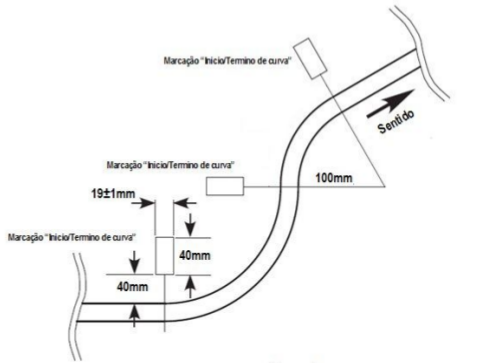
\includegraphics[scale=0.6]{figuras/Percurso4.png}
 \caption{Marcações de sinalização de curvatura \label{fig:percurso4}}
 \vspace{-0.3cm}
 \caption*{Fonte: Disponível em \cite[p.4]{RegrasRobocore}.}
\end{figure}


















